% !TeX encoding = UTF-8
% !TeX program = xelatex
\documentclass[12pt, a4paper]{article}
\usepackage{xeCJK} % 须放在\usepackage{}列中足够前的位置
\usepackage{fontspec}
\usepackage{graphicx}
\usepackage{caption}
\usepackage{enumerate}
\usepackage{setspace}
\usepackage{array} % 製作表格必須的宏包
\usepackage{tabularx} % 自動調整列寬的表格宏包
\usepackage{adjustbox}
\setCJKfamilyfont{heiti}{Heiti TC}
\CJKfamily{heiti}
\setmainfont{Arial}
\setstretch{1.5}


\begin{document}
\begin{center}
  {\Huge 邏輯設計實驗} \\[2.5cm]
  {\Huge Lab12} \\[1.5cm]
  {\Huge 非同步計數器} \\ [4.5cm]
  \hspace{.6in}
  \begin{minipage}[t]{.4\linewidth}
    {\Large 班級:資訊一甲}\\[0.5cm]
    {\Large 學號:D1109023}\\[0.5cm]
    {\Large 姓名:楊孟憲}
  \end{minipage}    
\end{center}

\newpage

\begin{description}
  \fontsize{22pt}{25pt}\selectfont 
    \item [一、]摘要 
      \begin{enumerate}
        \fontsize{20pt}{22pt}\selectfont
          \item 非同步計數器原理 \\
            \begin{samepage}
              \fontsize{16pt}{20}\selectfont
              每一級的時脈輸入會造成兩倍週期的Qi 輸出,而這個輸出又會當作下一級的時脈輸入,因此又造成兩倍週期的輸出\\
              \normalsize
              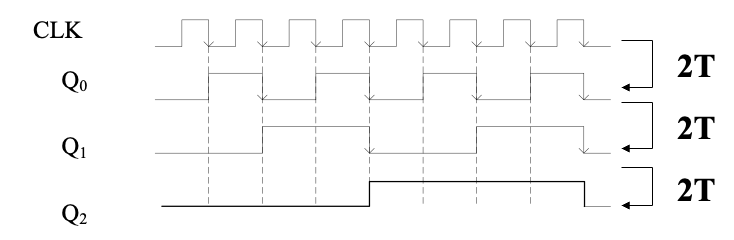
\includegraphics[width=13cm]{./image/截圖 2023-05-21 下午8.26.02.png}
            \end{samepage}

          \item Mod-N (模-N) 計數器/除N 除頻器 \\
            \begin{samepage}
              $\bullet$模 10 \\
              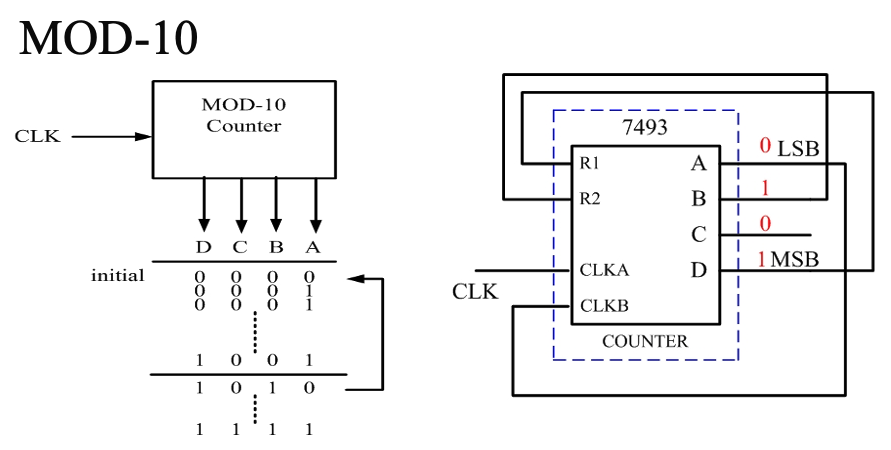
\includegraphics[width=13cm]{./image/n_mod.png}4
              \normalsize
            \end{samepage}
            
          \item 實驗 
            \begin{description}
              \fontsize{16pt}{20}\selectfont
                \item [(1)] 雙向4-bit計數器 
                \item [(3)] 利用7490設計一個 0~99 計數器 \\
              \normalsize  
            \end{description}
        \normalsize
      \end{enumerate}

    \item [二、]實驗結果
      \begin{description}
        \fontsize{20pt}{22pt}\selectfont
        \item 實驗一 (設計一個雙向4-bit計數器)
            \begin{description}
              \fontsize{18pt}{20pt}
                \item []電路圖 \\[.3cm]
                  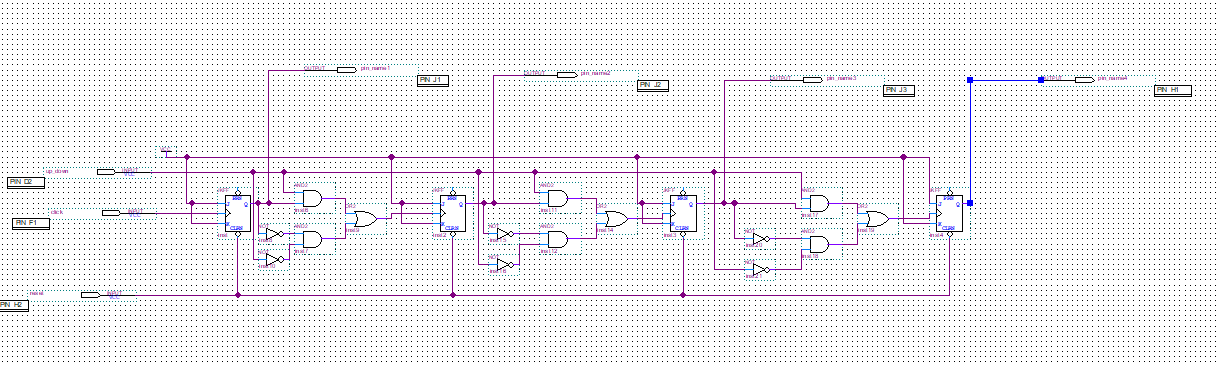
\includegraphics[width=13cm]{./image/ex1.png}
            \end{description}
          \normalsize
          
          \fontsize{20pt}{22pt}\selectfont
          \item 實驗二 (利用7490設計一個 0~99 計數器)
            \fontsize{16pt}{18pt}\selectfont
              \begin{description}
                \item [$\bullet$]請使用DE0所提供的 50MHz clock, CLOCK_50
                \item [$\bullet$] 將CLOCK_50 除頻 $10^7$,所得的 5Hz信號為此實驗的CLK\\
                \fontsize{18pt}{20pt}
                  \item []電路圖 \\[.3cm]
                    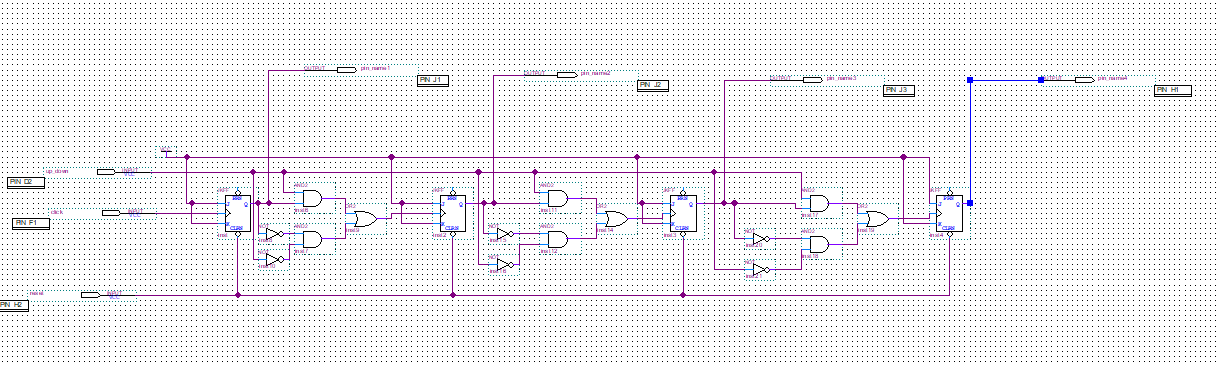
\includegraphics[width=13cm]{./image/ex1.png}
              \end{description}
            \normalsize
        \normalsize
      \end{description}
    \item [三、]問題討論心得 \\[.6cm]
      \begin{minipage}[t]{\linewidth}
        \fontsize{16}{18}\selectfont
        這次的實驗中,我成功地實作了一個雙向4-bit計數器,並利用7490芯片設計了一個0~99的計數器。整個實驗過程非常有趣且具有挑戰性。

        首先,我深入研究了7490芯片的功能和特性。7490是一個十進制計數器,能夠實現BCD(二進制編碼十進制)計數。我明白了7490的輸入和輸出的布局,並且瞭解了如何使用它來建構一個4位數計數器。
        
        在設計過程中,我學會了如何利用JK翻轉器和邏輯閘來建構每一位的計數器。我設置了四個JK翻轉器,每個翻轉器代表一個位元,從最低位元到最高位元。我透過適當的連接和設定,使得計數器能夠以二進制形式正確地計數,並且在達到最大值時從頭重新計數。
        \normalsize  
      \end{minipage}
  \normalsize
\end{description}

\end{document}


